\clearpage{}
\section{Define interfaces and classes in object-oriented design. Explain
typing and inheritance and the principles of polymorphism. Compare
inheritance and composition. Explain Liskov’s substitutability principle.
Explain and discuss the Law of Demeter. Describe the general principles and
constituting elements of design patterns.}

\subsection{Interfaces and classes in object-oriented design}

\begin{description}
    \item[Interface] Set of visible attributes and methods (signatures and specifications). It defines an abstract data type.
    \item[Class] Software module implementing an interface (i.e.\ it implements an abstract data type).
\end{description}

\subsection{Typing, inheritance and polymorphism}

\begin{figure}[!ht]
    \centering
    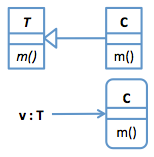
\includegraphics[width=0.2\linewidth]{inheritance.png}
\end{figure}

\subsubsection{Typing}

If $v: T$ refers to $o: C$
Static typing: only methods of $T$ can be invoked on $v$, checked at compilation.
Dynamic binding: when a method is invoked on $v$, the implementation of $C$ is executed,
checked at runtime.

\subsubsection{Inheritance}
Defining a new class (or interface) by reusing and extending an existing class (or interface).
A inherits from B iff A extends B iff A is a subtype of B.

\subsubsection{Polymorphism}
Different implementations from different classes $C$ are executed for the same invocation on $v$.
Ability of the code to act on values of multiple types.\newline
Improve the code reusability, e.g.\ implement one time a data structure such as list, array for
all the different data types.

\subsection{Comparison between inheritance and composition}

Two main techniques for constructing larger objects from smaller objects:

\begin{itemize}
    \item Inheritance: extend an existing class aka. White-box reuse. Use when subtyping is
useful.
    \item Composition: combine simpler classes aka. Black-box reuse. Preferred in general.
\end{itemize}

\begin{table}[!ht]
    \begin{tabular}{p{0.45\linewidth}p{0.45\linewidth}}
        Composition & Inheritance \\
        \begin{minipage}{\linewidth}
            \begin{center}
                \begin{tikzpicture}
    \umlemptyclass{Composite}
    \umlemptyclass[x=0, y=-2]{Component}
    \umlunicompo {Composite}{Component}
\end{tikzpicture}

            \end{center}

            \begin{itemize}
                \item[+] Only Composite interface is visible
                \item[+] Component can change dynamically
                \item[+] Multiple components is possible
                \item[+] Composite may use a Component
                interface
                \item[-] Component methods must be forwarded
                in Composite
                \item[-] Component unrelated to Composite
            \end{itemize}
        \end{minipage}
        &
        \begin{minipage}{\linewidth}
            \begin{center}
                \begin{tikzpicture}
    \umlemptyclass{Composite}
    \umlemptyclass[x=0, y=-2]{Component}
    \umlinherit {Composite}{Component}
\end{tikzpicture}

            \end{center}
            \begin{itemize}
                \item[+] Component methods invoked directly
                \item[+] Composite subtype of Component
                \item[-] Interface of Component is visible in
                Composite
                \item[-] Component fixed at design time
                \item[-] Only one Component is possible
                \item[-] Composite must extend a Component
                class
            \end{itemize}
        \end{minipage}
    \end{tabular}
\end{table}

\subsection{Liskov’s substitutability principle}

\begin{figure}[!ht]
    \centering
    \begin{tikzpicture}
    \umlemptyclass{Subclass}
    \umlemptyclass[x=0, y=-2]{Superclass}
    \umlinherit {Subclass}{Superclass}
\end{tikzpicture}

\end{figure}

\subsubsection{Substitutability}

\begin{itemize}
    \item Subclass is a subtype of Superclass
    \item Subclass instances can be used as Superclass instances
    \item Subclass must preserve the behaviour of Superclass
    \item Subclass must respect the contract of Superclass, so that Subclass instances are substitutable to Superclass instances
\end{itemize}

N.B. this is a guiding principle, not an absolute rule. \newline

\subsubsection{Liskov’s substitutability principle}

Subclass is substitutable for Superclass if:

\begin{enumerate}
    \item Subclass supports all the methods of Superclass (with compatible signatures)
    \item Subclass methods satisfy the specifications of Superclass methods
    \item Subclass preserves all properties of Superclass
\end{enumerate}

\subsection{Law of Demeter (aka. \enquote{Don't talk to strangers})}

Each unit should have knowledge only on directly related units. \newline
In OO programming: each class should invoke methods only on directly referenced classes.

\begin{itemize}
    \item[+] Reduces dependencies
    \item[+] Client of a composite need not know its components
    \item[-] Needs additional wrapper functions, may degrade performance
\end{itemize}

\subsection{General principles and constituting elements of design patterns}

A design pattern codifies design decisions and practices for solving a particular design
problem according to design principles. \newline

They are templates for a solution that must be modified and adapted for each particular use. \newline

Elements of a design pattern:

\begin{description}
    \item[Name] for easy reference, enriches our design vocabulary
    \item[Problem] when to apply, objectives
    \item[Solution] structure, elements and relationships
    \item[Consequences] benefits and costs, trade-offs
\end{description}
